\documentclass[a4paper]{article}

\usepackage[english]{babel}
\usepackage[utf8]{inputenc}
\usepackage{amsmath}
\usepackage{graphicx}
\usepackage[colorinlistoftodos]{todonotes}
\usepackage{float}


\title{Calcul de descripteurs locaux et de dictionnaires visuels}

\author{Florian Toqué}

\date{\today}

\begin{document}
\maketitle

\begin{abstract}

Ce rapport porte sur un travail effectué au cours de l'UE RDFIA du Master informatique spécialité Imagerie de l'université Pierre et Marie Curie (Paris). Le travail réalisé consiste à mettre en place un système de classification d’images par apprentissage supervisé. Une fois appris ce système de classification est en mesure d’affecter une des 15 cateégories sémantiques à une image de test donnée. Dans ce rapport nous expliquons  les différentes parties nécessaire à l'élaboration de ce système de classification. 
\end{abstract}

\section{Introduction}
Lors de ce projet nous avons implémenté deux parties, le calcul des descripteur SIFT de la base d'image et la création de dictionnaire visuel permettant de définir une image à l'aide de "mots" de ce dictionnaire.


\section{Descripteurs locaux : SIFT }
Pour analyser les images il est nécessaire d'avoir un moyen de représenter l'information contenue dans celles-ci. Pour ce faire nous utilisons un descripteur SIFT (Scale-Invariant Feature Transform)  correspondant aux caractéristiques d'une partie de l'image, l'image sera donc représentée par un ensemble de descripteurs SIFT. 
\subsection{Calcul du descripteurs SIFT pour une région (patch)}
Un descripteur SIFT correspond à une région de taille 16x16 pixels de l'image. Il est de taille 128 et représente de manière concaténée, les histogrammes représentant l'information sur une partie du patch(4x4 pixels). Ces histogrammes étant calculé a l'aide de gradient en chaque pixel pondérés par un masque gaussien centrée sur les points d'intérêts. Ce descripteur permettra de comparer deux régions de deux images en fonction des formes qu'ils représentent, formes ou contours captés grâce aux différences de contrastes, calculées à l'aide de gradients.\\

Question: Montrer que les masques Mx (resp. My) sont séparables, c'est à dire qu'ils peuvent s’écrire comme Mx = hy x hx , où hy est un masque 1d sur les lignes (taille 3 x 1) et hx est un masque 1d sur les colonnes ( taille 1 x 3 ).\\

Réponse: On a hx = [-1 0 1]; et hy = [1;2;1]; on a bien hy x hx = Mx.\\

Explication en image:\\
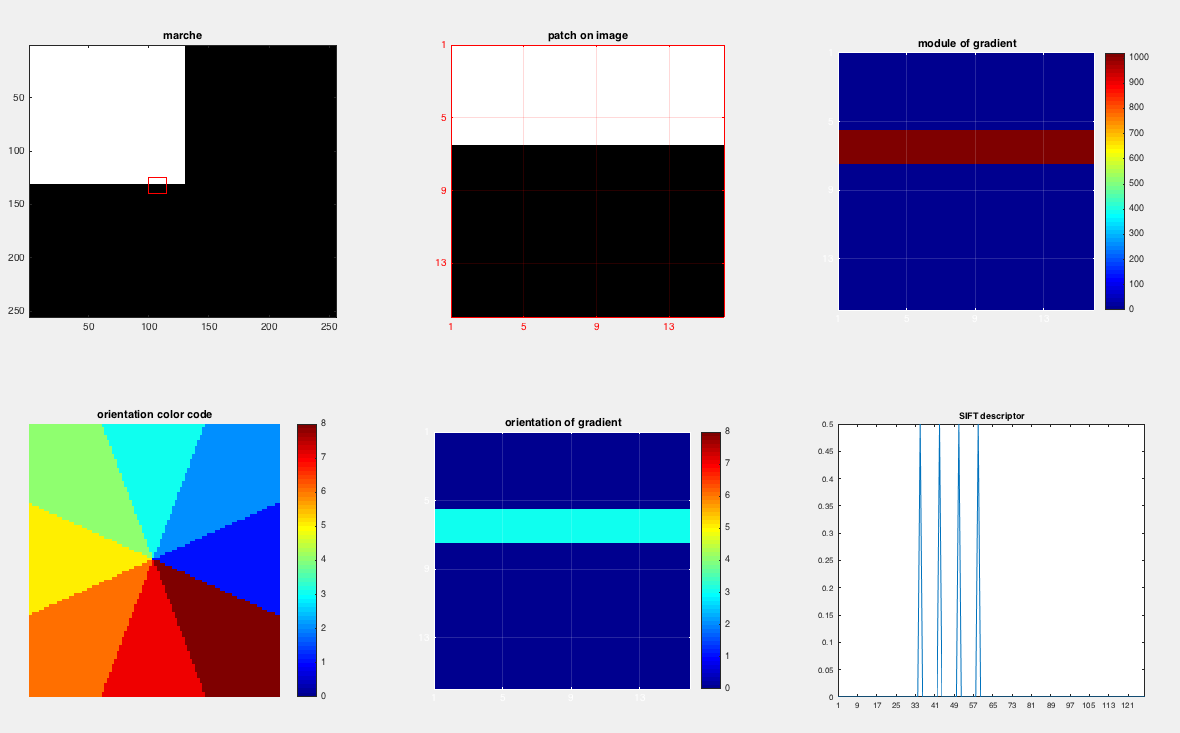
\includegraphics[width=\textwidth]{Sift_patch_marche}\\\\
On remarque bien que le gradient est fort au niveau de la frontière blanc/noir. Le patch à donc détecté un contour. Le descripteur SIFT de taille 128 contient les histogrammes de manière concaténé, voila pourquoi on observe des pique sur les abscisses 5,6,7,8, qui correspondent aux histogrammes de la deuxième ligne du descripteur.\\

Image marche (pixel x97 y 121)\\\\
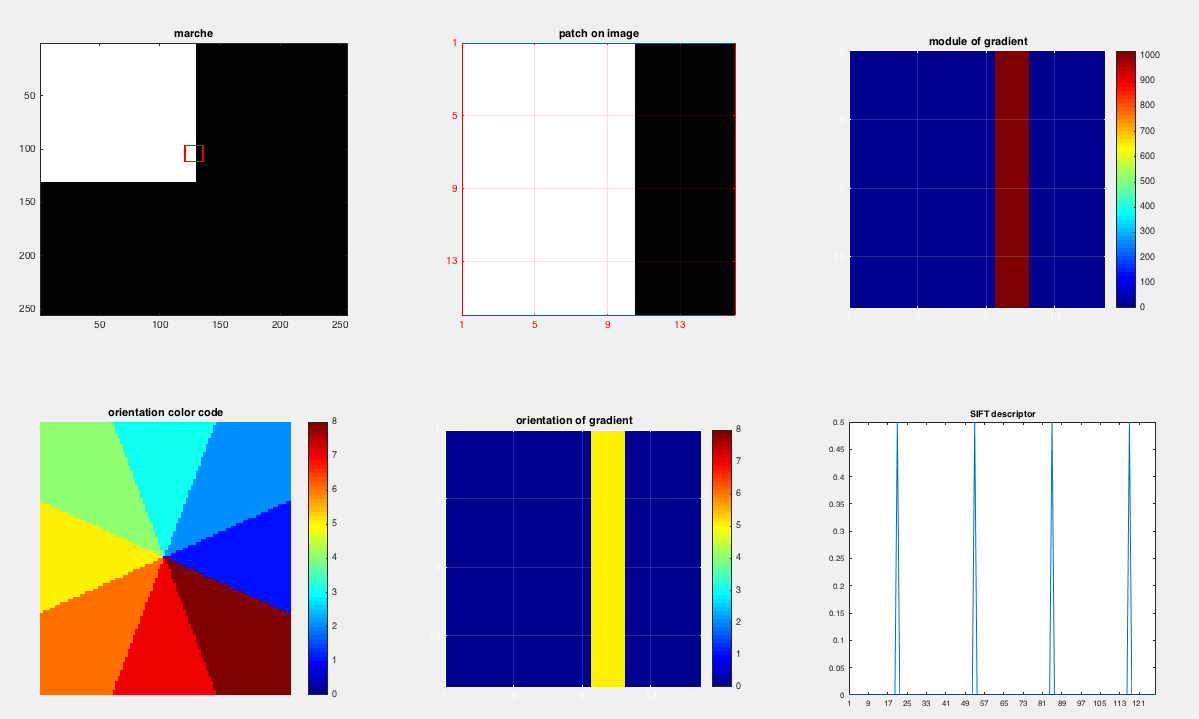
\includegraphics[width=\textwidth]{marche_97_121}\\

Image marche (pixel x121 y 121)\\
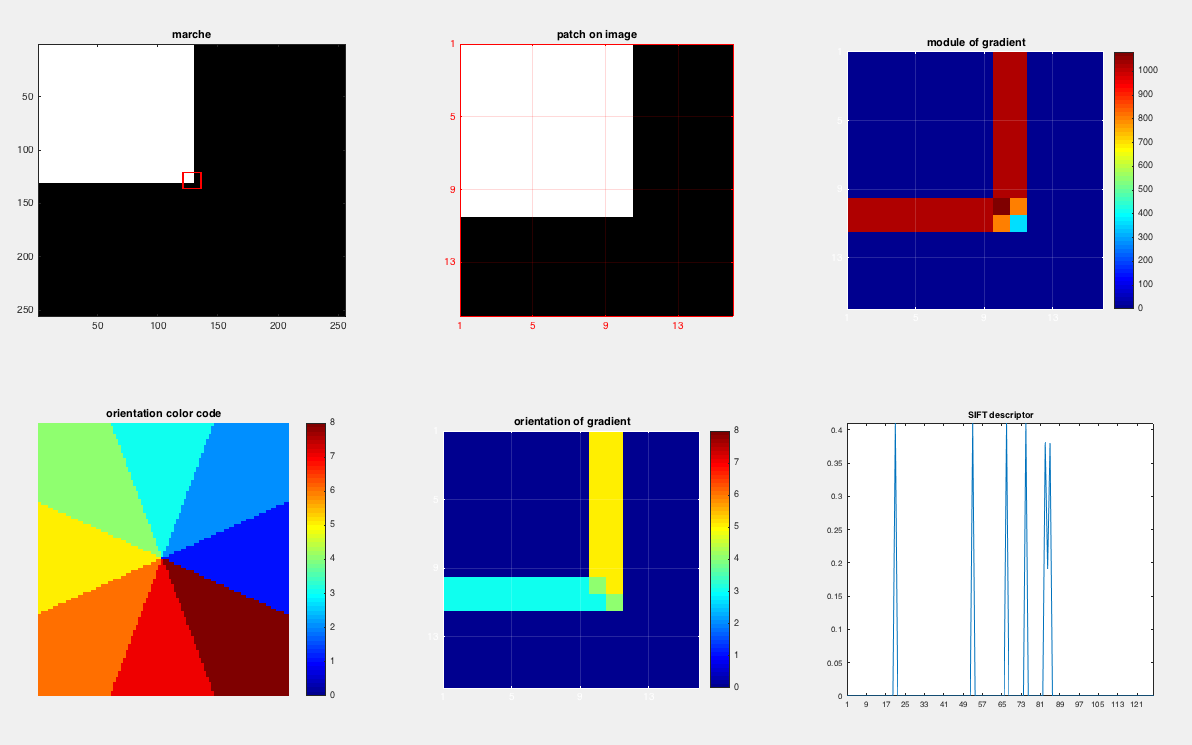
\includegraphics[width=\textwidth]{marche_121_121}\\

Image tools\\
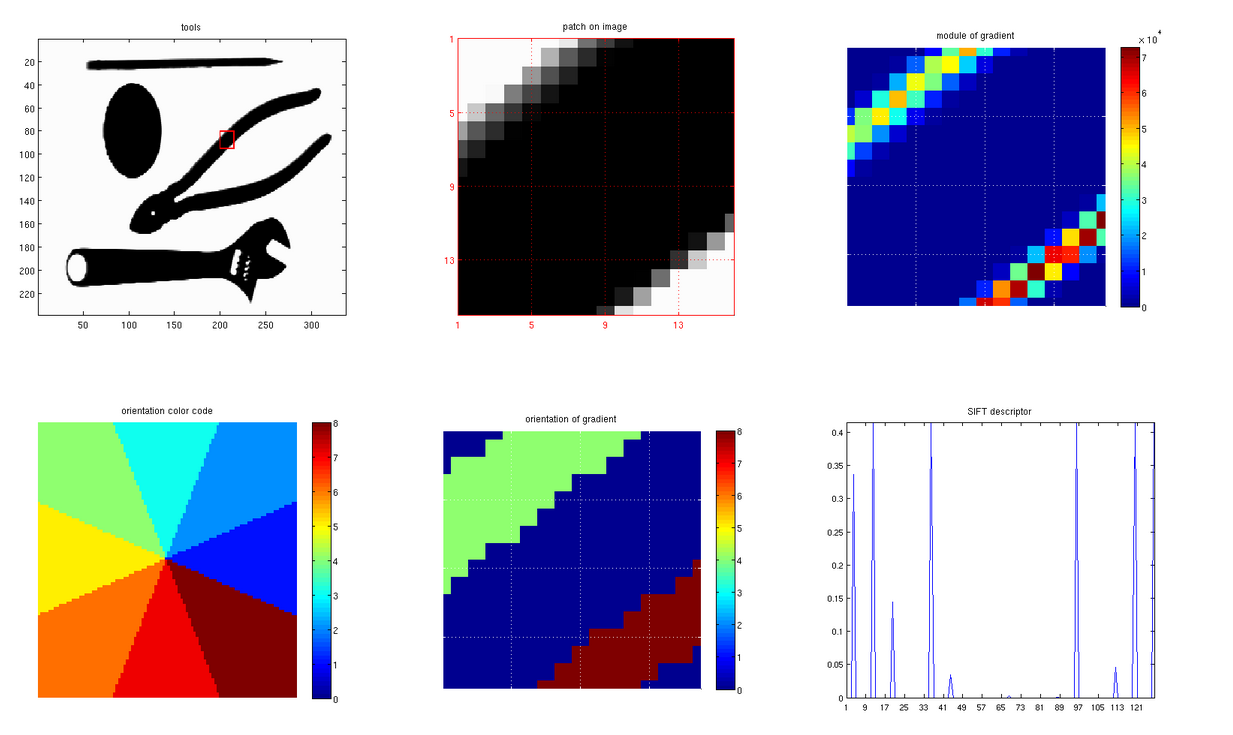
\includegraphics[width=\textwidth]{tools_80}
\\
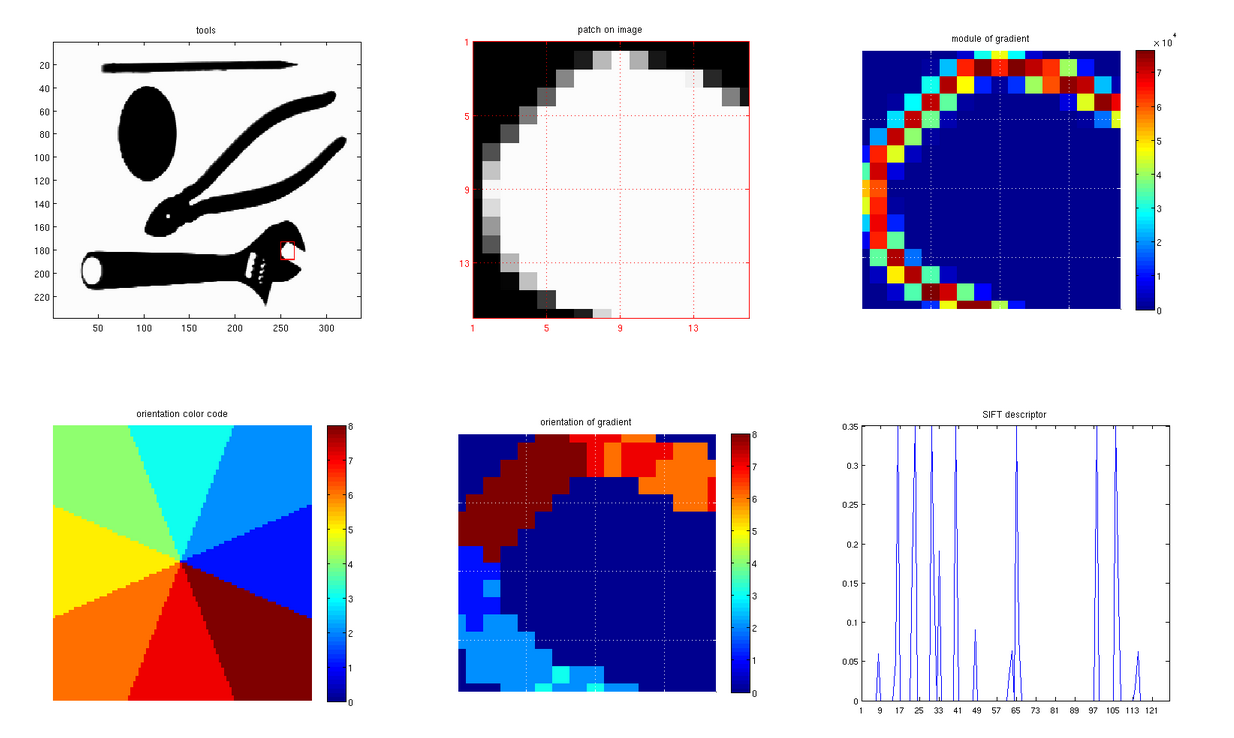
\includegraphics[width=\textwidth]{tools_173}\\
Dans ces deux dernières images nous remarquons que le gradient est plus élevé lorsque le contraste l'est aussi et que cette information est bien retranscrite dans le descripteur SIFT.\\
\\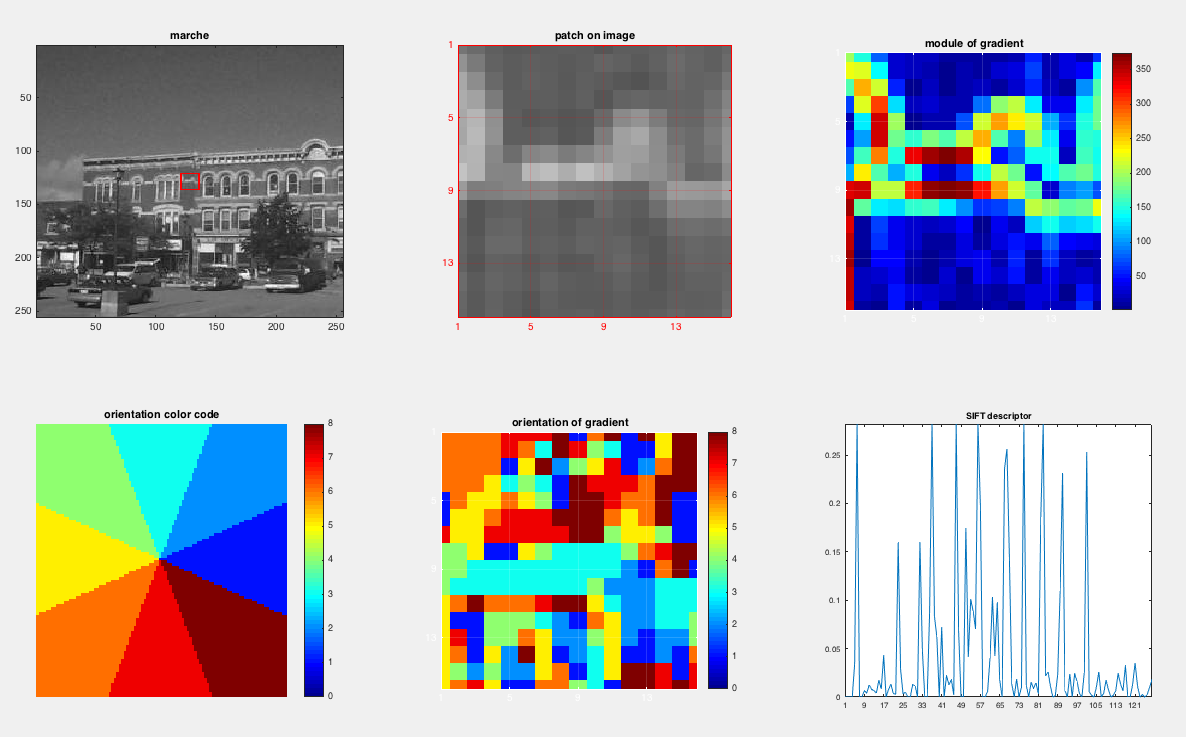
\includegraphics[width=\textwidth]{sift}\\\\\\
Nous pouvons facilement voir que dans cette image le SIFT associé à la partie entourée en rouge, représente un élément de l'image ayant une forme intéressante ici puisque les gradients ont une forte valeur. En effet il s'agit d'une partie composant un mur de façade, partie qui pourra etre utilisée pour la classification d'image.

\subsection{Calcul des descripteurs SIFT pour une image}
Ces Sifts sont normalisés plusieurs fois. Le fait de normaliser les sifts ajoute un problème celui des régions homogènes en effet nous ne voulons pas prendre en compte les variations de contraste dans ces régions. A cause de la normalisation, ces variations sont tout de même prises en compte il est donc nécessaire de seuillé les patch avant la normalisation. Ainsi les régions homogène avec de faibles gradient (en dessous de 0.2) seront représentés par des SIFT nuls. Nous obtenons alors ce type de résultats: les patch bleus représentent des régions homogènes et donc des régions sans intérêt contrairement aux patchs rouges qui eux contiennent de l'information utiles (SIFT non nuls).\\
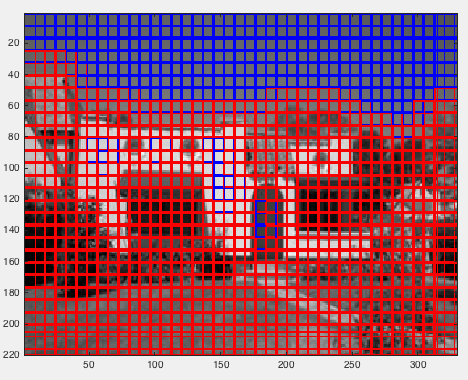
\includegraphics[width=\textwidth]{versionrougebleu}\\

\subsection{Calcul de l’ensemble des descripteurs de la base}
Afin d'avoir la représentation de chaque image nous enregistrons dans un fichier tous les SIFT de chaque image. \\
La différence avec l'algorithme de Lowe et le notre est que nos SIFT sont normalisés,seuillés puis renormalisés, contrairement aux SIFT de Lowe qui ne sont que normalisés. Cette astuce permet de repérer la même forme que ce soit sur une image prise de jour (luminosité forte) ou de nuit(luminosité faible), ce qui est très utile en classification d'image. L'accent est mis sur la forme peut importe la luminosité de l'image.

\section{Génération de dictionnaire visuel}
Afin de minimiser la distorsion des données et donc de réduire l'espace de comparaison entre différentes images, nous créons un dictionnaire visuel comportant des mots qui représentent ou en tout cas se rapprochent des descripteurs SIFT ,de notre base d'image. Pour se faire nous utilisons l'algorithme des K-means permettant de regrouper autour de barycentres des descripteurs SIFT qui sont proches entre eux.

\subsection{Quantification et K-Means}
L'algorithme du K-Means vise à minimiser la fonction de coût qui est la somme des distances des points d'un cluster à leur barycentre. Si un barycentre est trouvé pour un cluster, étant donné qu'il minimise la distance avec tous ses autres points, il n'est pas possible de trouver un autre point qui minimise cette distance. On a donc bien le barycentre qui minimise la distorsion des données.

\section{Conclusion}
A l'aide des descripteurs SIFT et d'une manière de les représentés en minimisant la distorsion des données nous avons appris à représentés l'information des images de manière compacte et simple à utiliser pour faire des calculs de distances de manière automatique entre plusieurs images et ainsi réussir à faire de la classification.
\end{document}